
% ------------------------------------------------------------
% ------------------------------------------------------------

%%%%%%%%%%%%%%%%%%%%%%%%%%%%%%%%%%%%%
\section{3D Plots}
\subsection{\ttfamily lattice \normalfont library}

%%%%%%%%%%%%%%%%%%%%%%%
\begin{frame}[fragile]
\frametitle{3D Images with Package \ttfamily lattice \normalfont}

\vspace{0.1in}
\bf{Method 1:} \normalfont Using \ttfamily wireframe(): \normalfont 

    \begin{columns}
      \column{0.50\textwidth}
\begin{lstlisting}
library(lattice)
wireframe(volcano, col.regions = terrain.colors(100), asp = 1, color.key=TRUE, drape=TRUE, scales = list(arrows = FALSE))
\end{lstlisting}
%g <- expand.grid(x = 1:10, y = 5:15)
%g$z<-g$x^2
%wireframe(g$z~g$x*g$y, scales = list(arrows = FALSE), drape = TRUE, colorkey = TRUE)

     \column{0.50\textwidth}
       \begin{center}
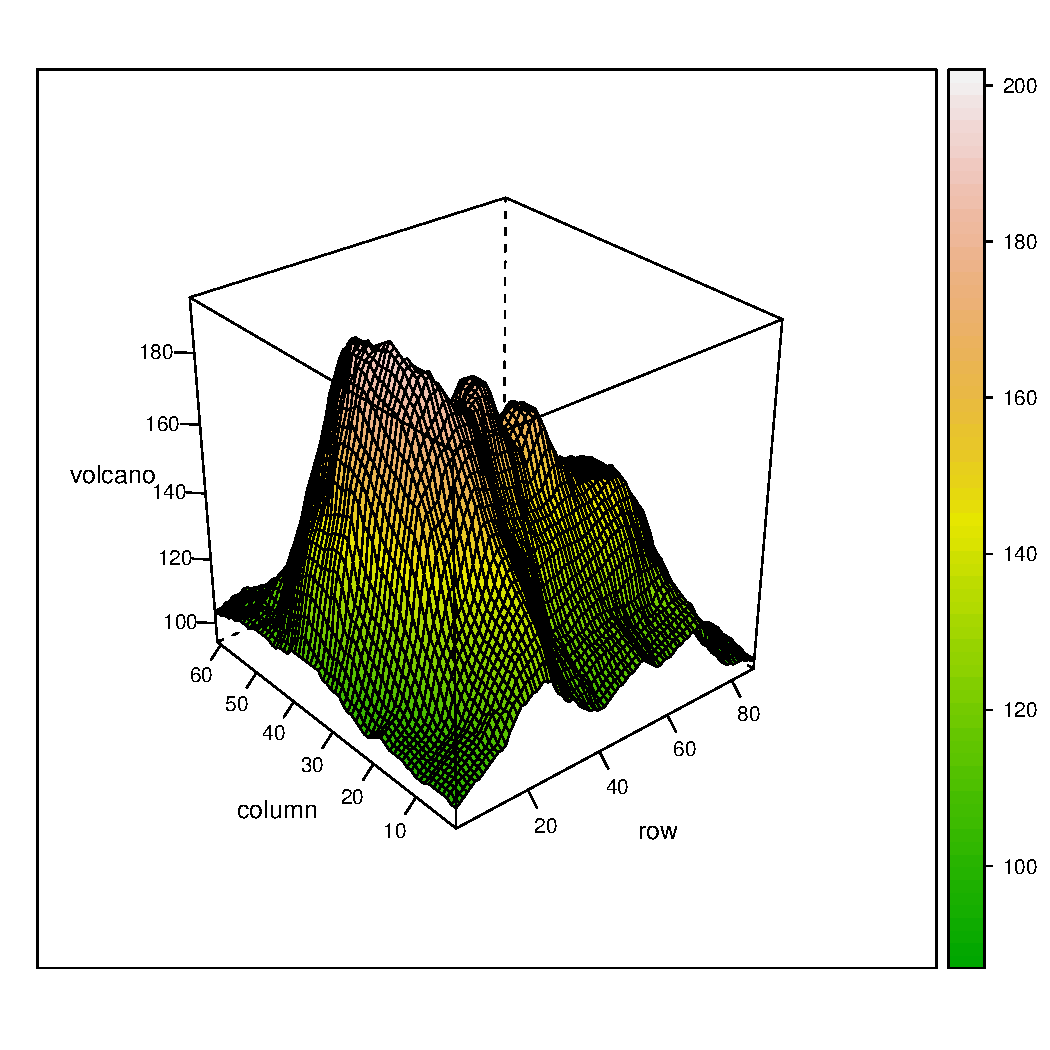
\includegraphics[width = 55mm]{images/wireframe.pdf}
\end{center}
\end{columns}
\end{frame}

%%%%%%%%%%%%%%%%%%%%%%%
\begin{frame}[fragile]
\frametitle{3D Images with Package \ttfamily lattice \normalfont}

\bf{Method 2:} \normalfont Same image with the \ttfamily levelplot() \normalfont function:

    \begin{columns}
      \column{0.50\textwidth}
\begin{lstlisting}
library(lattice)
levelplot(volcano, asp=1, col.regions=terrain.colors)
\end{lstlisting}

     \column{0.50\textwidth}
       \begin{center}
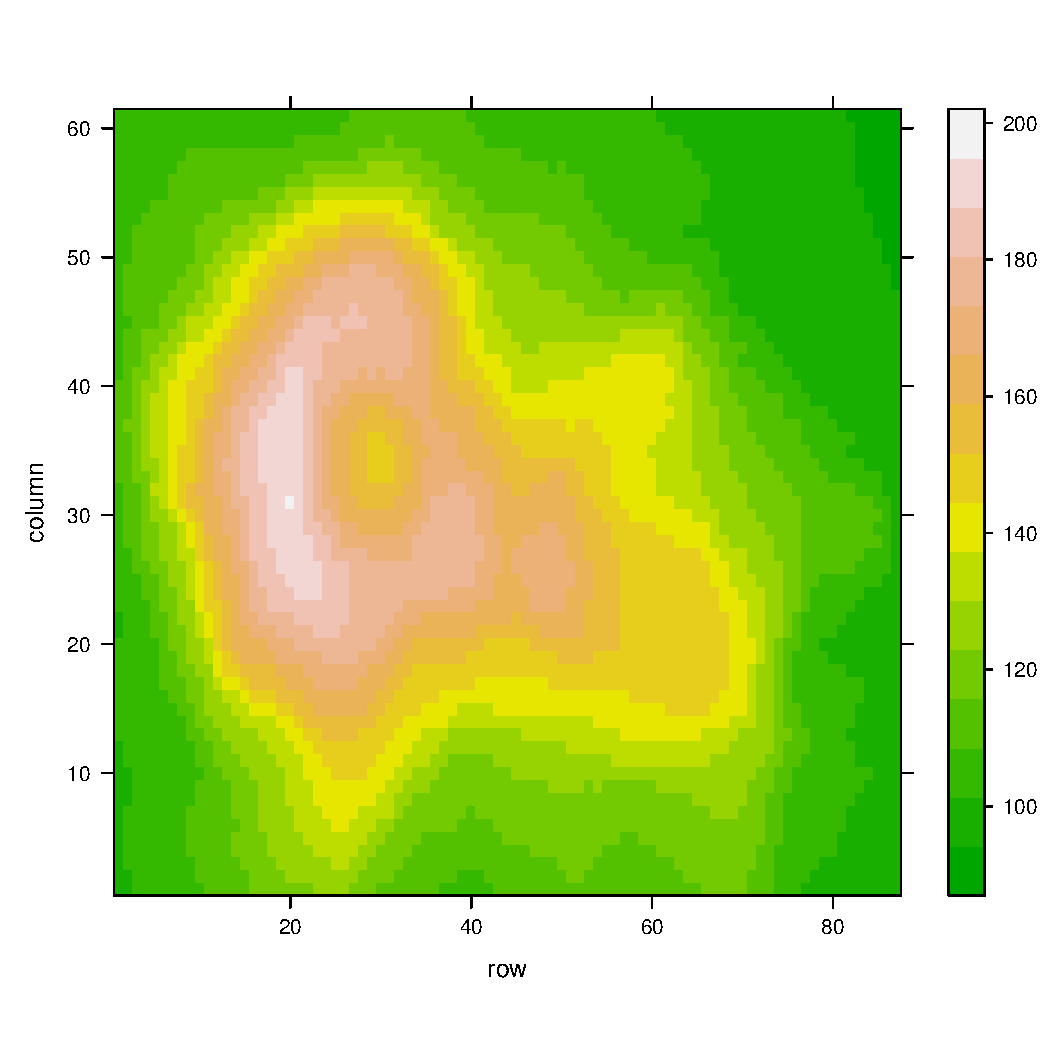
\includegraphics[width = 55mm]{images/levelplot.pdf}
\end{center}
\end{columns}
\end{frame}

%%%%%%%%%%%%%%%%%%%%%%%
\begin{frame}[fragile]
\frametitle{3D Images with Package \ttfamily lattice \normalfont}

\bf{Method 3:} \normalfont Same image with the \ttfamily image() \normalfont function:
    \begin{columns}
      \column{0.52\textwidth}
      
\begin{lstlisting}
x<-10*(1:nrow(volcano))
y<-10*(1:ncol(volcano))
image(x, y, volcano, col = terrain.colors(100), axes = TRUE)
contour(x, y, volcano, add = TRUE, col = 1)
\end{lstlisting}

     \column{0.48\textwidth}
       \begin{center}
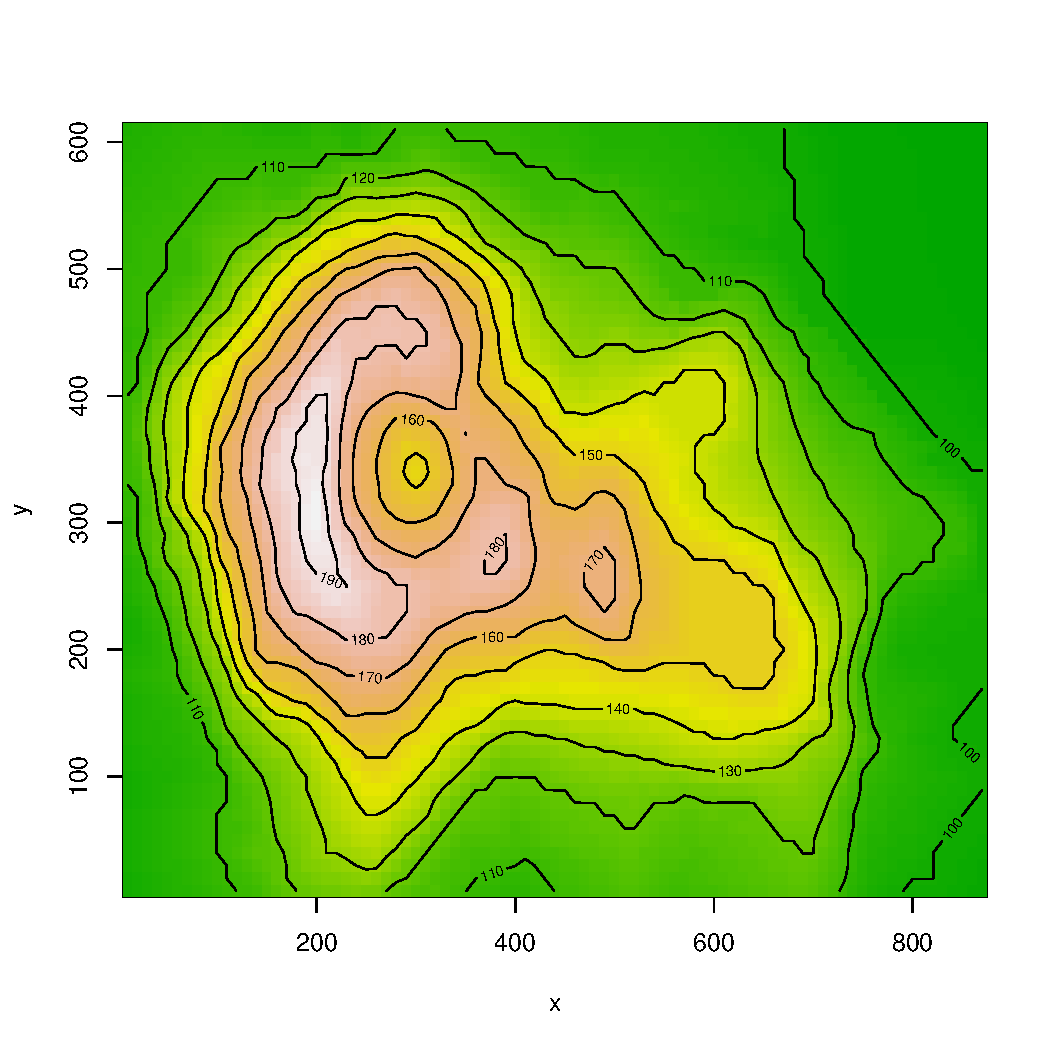
\includegraphics[width = 55mm]{images/image.pdf}
\end{center}
\end{columns}
\end{frame}
% plot3d(iris)

%%%%%%%%%%%%%%%%%%%%%%%
\subsection{\ttfamily ggplot2 \normalfont library} 
%%%%%%%%%%%%%%%%%%%%%%%
\begin{frame}[fragile, allowframebreaks]
\frametitle{3D Images with Package \ttfamily ggplot2 \normalfont}

Another way to create 3D images is with the package \ttfamily ggplot2: \normalfont 

%\bf{Method 1:} \normalfont Using \ttfamily wireframe(): \normalfont 
\begin{lstlisting}
# Step 1: Load the data
data(quakes)
attach(quakes)
# Step 2: Create a categorical variable for earthquake magnitude
ind<-which(mag<5)
ind2<-which(mag<6 & mag >=5)
ind3<-which(mag>=6)
color<-rep(NA, length(mag))
color[ind]<-1; color[ind2]<-2; color[ind3]<-3
color<-as.factor(color)


# Step 3: Plot
library(ggplot2)
ggplot(data=quakes, aes(long, lat))+
	geom_point(aes(long, lat))+
	borders("world")+
	coord_cartesian(xlim=c(100,190), ylim=c(-40,0))
\end{lstlisting}

\newpage
       \begin{center}
		\includegraphics[scale=0.22]{images/ggplotPlot1.pdf}
	\end{center}
\end{frame}

\begin{frame}[fragile, allowframebreaks]
\frametitle{3D Images with Package \ttfamily ggplot2 \normalfont}

To include information on magnitude of earthquake, use \ttfamily geom\_point(): \normalfont 

%\bf{Method 1:} \normalfont Using \ttfamily wireframe(): \normalfont 
\begin{lstlisting}
ggplot(data=quakes, aes(long, lat))+
	borders("world")+
	coord_cartesian(xlim=c(100,190), ylim=c(-40,0))+	
	geom_point(data=quakes, colour=as.numeric(color), size=2*as.numeric(color))
\end{lstlisting}

\newpage
       \begin{center}
		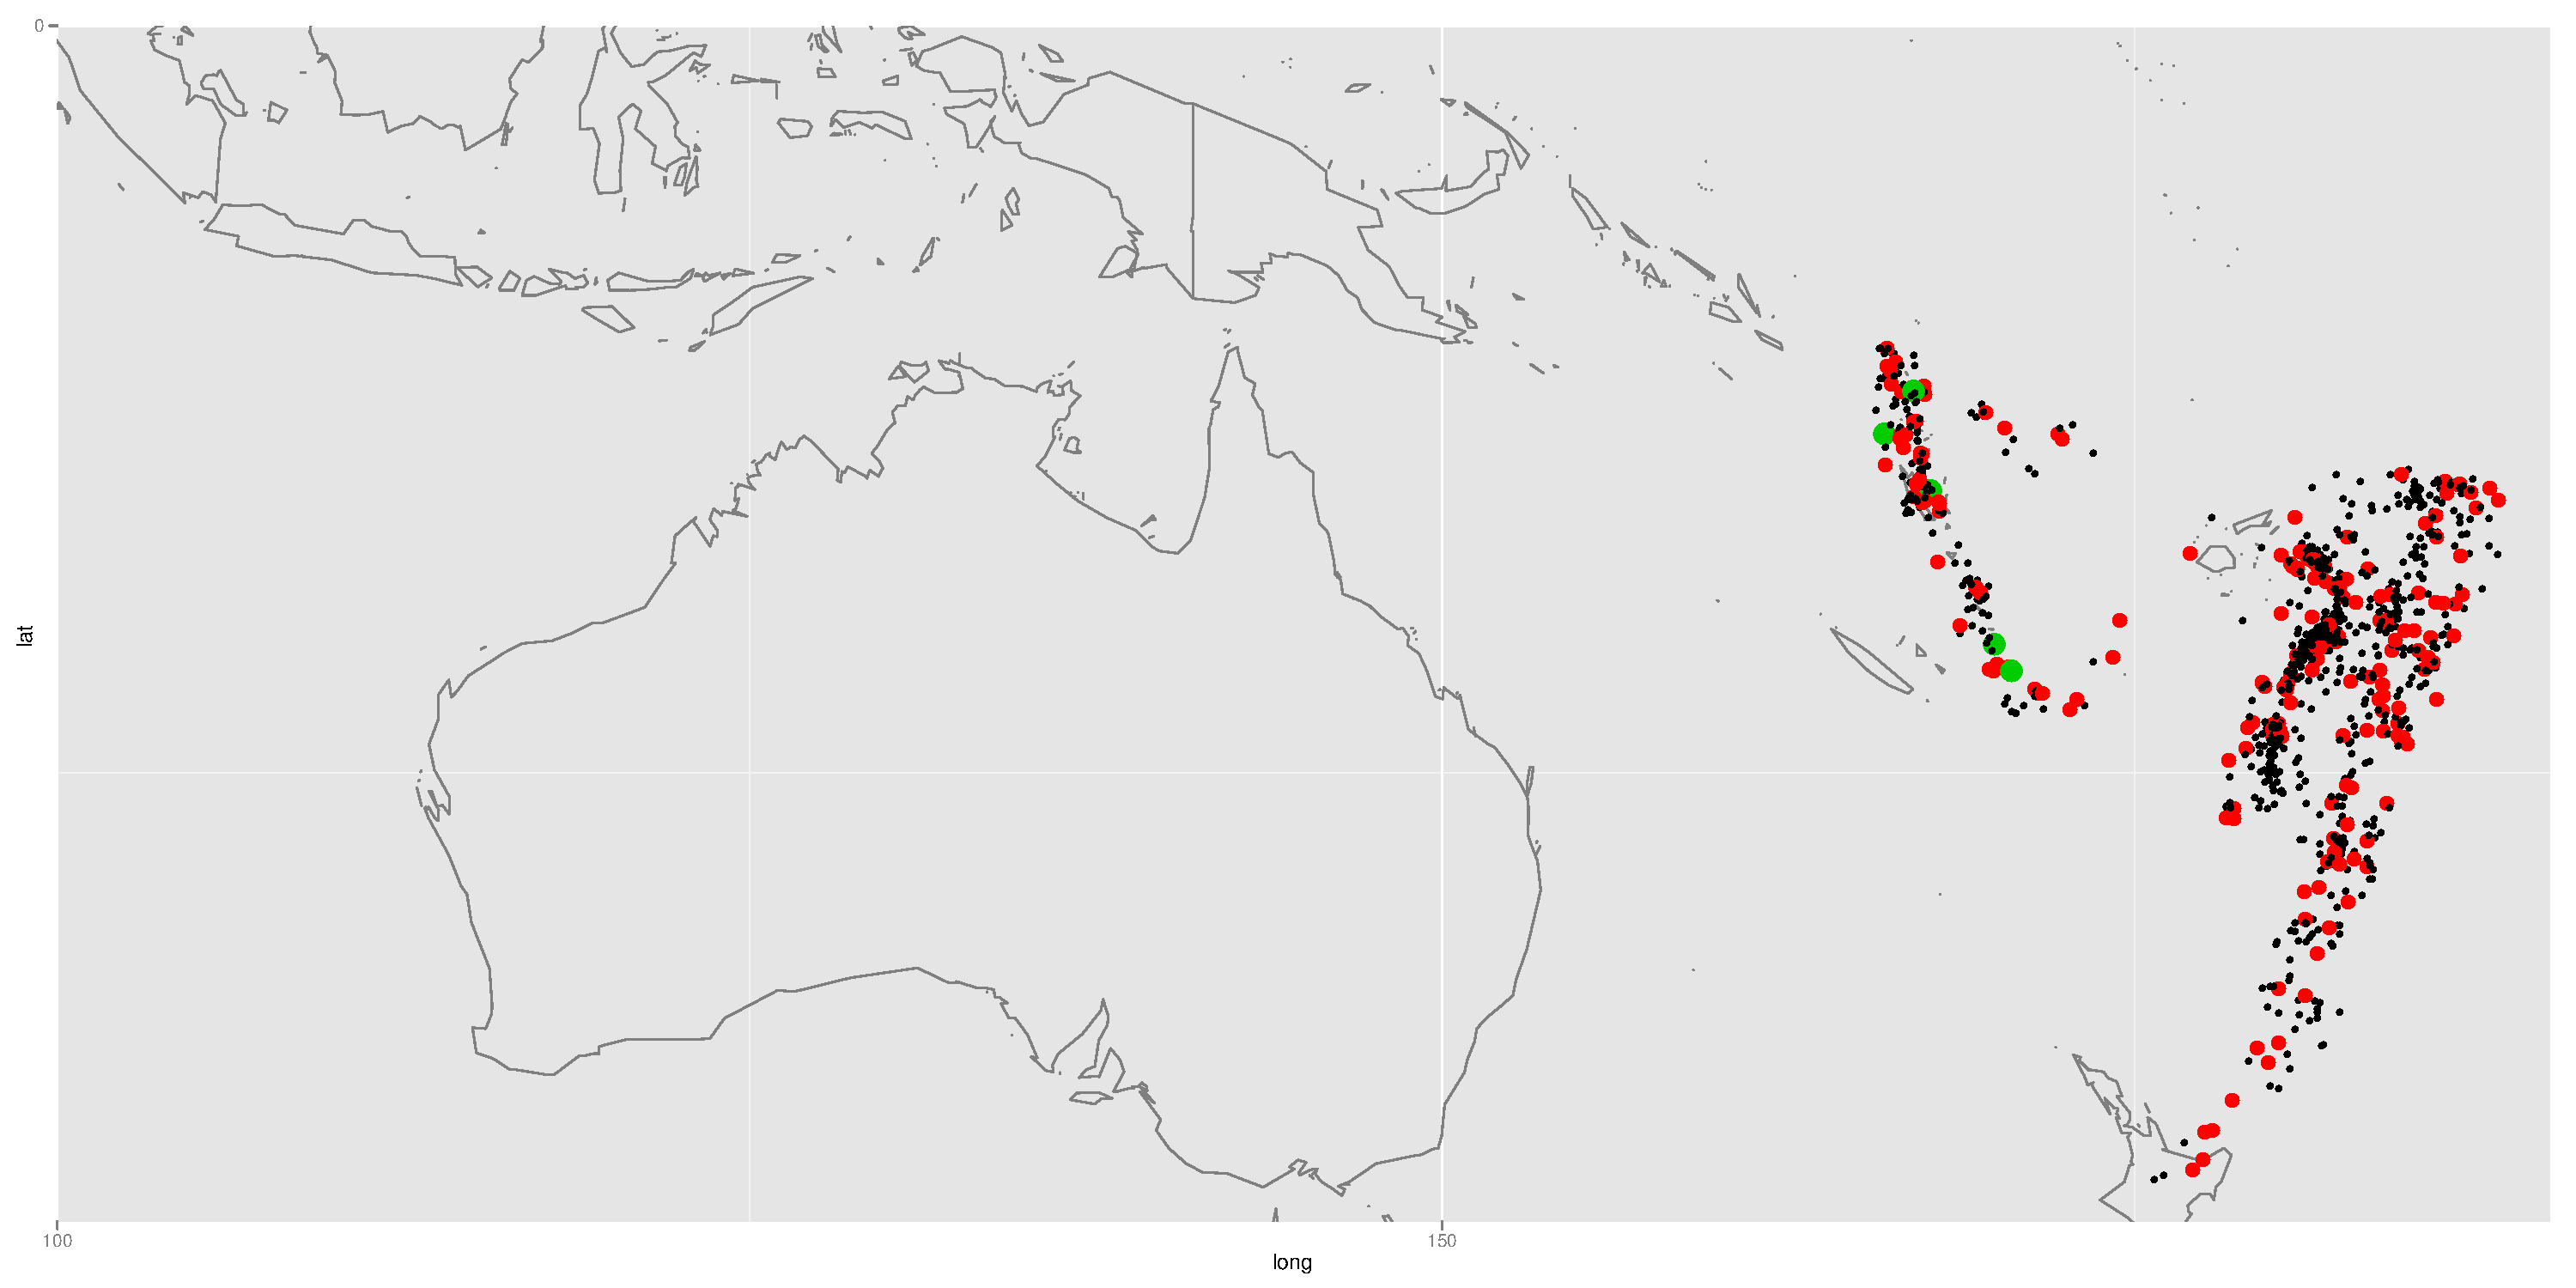
\includegraphics[scale=0.22]{images/ggplotPlot2.pdf}
	\end{center}
\end{frame}


%%%%%%%%%%%%%%%%%%%%%%%
\subsection{\ttfamily rgl \normalfont library} 
%%%%%%%%%%%%%%%%%%%%%%%
\begin{frame}[fragile]
\frametitle{3D Images with Package \ttfamily rgl \normalfont}

A way to create 3D interactive images is with the package \ttfamily rgl: \normalfont 

    \begin{columns}
      \column{0.50\textwidth}
\begin{lstlisting}
library(rgl)
data(quakes)
plot3d(x=quakes[, 2], y=quakes[, 1], z=quakes[, 3], xlab="Longitude", ylab="Latitude", zlab="Depth")
\end{lstlisting}
%g <- expand.grid(x = 1:10, y = 5:15)
%g$z<-g$x^2
%wireframe(g$z~g$x*g$y, scales = list(arrows = FALSE), drape = TRUE, colorkey = TRUE)

     \column{0.50\textwidth}
       \begin{center}
\includegraphics[width = 55mm]{images/Fiji_RGL}
\end{center}
\end{columns}
\end{frame}

%%%%%%%%%%%%%%%%%%%%%%%
\subsection{Saving Plots as a PDF} 
%%%%%%%%%%%%%%%%%%%%%%%
\begin{frame}[fragile]
\frametitle{Saving Plots as a PDF}
\framesubtitle{For Static Plots}

\itshape Note: \normalfont The files will be saved in the folder specified with \ttfamily setwd(). \normalfont
To save a static plot in \ttfamily R \normalfont as a PDF, use function \ttfamily pdf(): \normalfont

\begin{lstlisting}
# To save the image to the desktop:
setwd("~/Desktop")
wireframe(volcano, col.regions = terrain.colors(100), asp = 1, color.key=TRUE, drape=TRUE, scales = list(arrows = FALSE))
dev.off()
\end{lstlisting}

\end{frame}

\begin{frame}[fragile]
\frametitle{Saving Plots as a PDF}
\framesubtitle{For Dynamic Plots}

\itshape Note: \normalfont The files will be saved in the folder specified with \ttfamily setwd(). \normalfont
To save a dynamic plot in \ttfamily R \normalfont as a PDF, use function \ttfamily rgl.snapshot(): \normalfont

\begin{lstlisting}
# To save the image to the desktop:
setwd("~/Desktop")
# Step 1: Produce the 3D image:
plot3d(x=quakes[, 2], y=quakes[, 1], z=quakes[, 3], xlab="Longitude", ylab="Latitude", zlab="Depth")
# Step 2: Can rotate before taking a snapshot:
rgl.snapshot("quakes.png")
\end{lstlisting}

\end{frame}



% ------------------------------------------------------------
% ------------------------------------------------------------
\subsection{Exercise IV}
\begin{frame}
	\frametitle{Exercise IV}
	Use the \ttfamily rgl \normalfont library to create a 3D plot of the \ttfamily ozone \normalfont data set \footnote{\ttfamily http://www.ats.ucla.edu/stat/R/faq/ozone.csv\normalfont}.
\end{frame}